\documentclass[12pt,a4paper]{article}
\usepackage[OT1]{fontenc}
\usepackage{amsmath}
\usepackage{amsfonts}
\usepackage{amssymb}
\usepackage{graphicx}
\usepackage{array}
\usepackage{cancel}
\usepackage{caption}
\usepackage{wrapfig}
\usepackage{secdot}
\usepackage{indentfirst}
\usepackage{mathrsfs}
\usepackage[left=1.5cm,right=1.5cm,top=0.3cm,bottom=1.5cm,includefoot,footskip=1.5cm]{geometry}
\usepackage[utf8]{inputenc}
\usepackage[english, russian]{babel}
\begin{document}
\textbf{
\begin{flushright}
Илья Кочергин, 626 группа
\end{flushright}}
\paragraph{\large Работа 3.4.5}
\paragraph{\Large Петля гистерезиса}
\paragraph{Цель работы:}изучение петель гистерезиса ферромагнитных материалов с помощью осциллографа.
\paragraph{Оборудование:}понижающий трансформатор, реостат, резистор, интегрирующая цепочка, амперметр и вольтметр (мультиметры), электронный осциллограф, делитель напряжения, переключатель, тороидальные образцы с двумя обмотками.
\section{Теоретическая справка}
\paragraph{Гистерезис.} У ферромагнитных материалов зависимость индукции магнитного поля от напряженности ($B(H)$) не является линейной. Кроме того, даже при отсутствии магнитного поля сохраняется остаточная намагниченность. Поэтому важно знать вид этой зависимости. Будем использовать следующие понятия: $B_r = B(H = 0)$~--- остаточная индукция, $H_c = -H(B = 0)$~--- коэрцитивная сила, максимальная возможная индукция магнитного поля $B_s$~--- индукция насыщения (при достижении некоторого значения $H$ индукция перестает увеличиваться). При этом предполагается, что $H$ сначала увеличивается из состояния с нулевой намагниченностью, а потом уменьшается (возврат происходит по другой кривой). Определим также дифференциальную магнитную проницаемость $\mu_\text{дифф}$:
\begin{equation}
\mu_\text{дифф} = \frac{1}{\mu_0}\frac{dB}{dH}.
\end{equation}
\paragraph{Способ измерения индукции.} Пусть на образец намотана катушка с числом витков $N$ и площадью $S$. Тогда в силу закона Фарадея индукция определяется формулой
\begin{equation}
|B| = \frac{1}{SN}\int\mathscr{E} dt,
\end{equation}
где $\mathscr{E}$~--- наводимая ЭДС. Для интегрирования сигнала используется интегрирующая цепочка, состоящая из резистора с большим сопротивлением $R$, соединенного последовательно с конденсатором емкостью $C$. Выходной сигнал $U$ снимается с конденсатора. Если сопротивление достаточно большое, то выходной сигнал определяется выражением
\begin{equation}
U = \frac{q}{C} = \frac{1}{C}\int Idt \approx \frac{1}{RC}\int U_0 dt,
\end{equation}
где $U_0$~--- входное напряжение. В случае синусоидальных напряжений интеграл тривиален, и формула (2) принимает вид
\begin{equation}
|B| = \frac{RC}{SN}U.
\end{equation}
Для проверки корректности использования этой формулы можно измерить постоянную времени $RC$. Из (3) должно выполняться соотношение
\begin{equation}
RC = \frac{U_0}{\Omega U},
\end{equation}
где $\Omega$~--- циклическая частота сигнала.
\newpage
\section{Калибровка осей осциллографа}
\begin{wrapfigure}{r}{0.45\textwidth}
\centering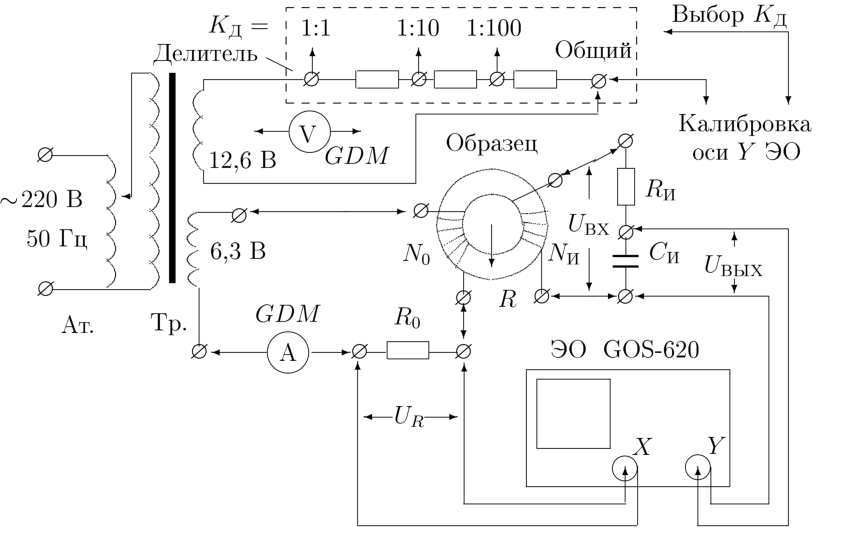
\includegraphics[width = 0.45\textwidth]{Pct1}
\captionsetup{justification = centering}
\caption{Схема установки \label{Pct}}
\end{wrapfigure}
\paragraph{Экспериментальная установка.} На рисунке 1 представлена общая схема экспериментальной установки. В этой части определяются чувствительности каналов осциллографа, поэтому полная схема не используется. Для определения чувствительности $X$~--- канала обмотка $N_0$ закорачивается и снимаются показания тока $I$ через резистор $R_0 = 0,3$ Ом с амперметра $A$. Тогда чувствительность $X$~--- канала определяется формулой
\begin{equation}
m_x = \frac{2R_0\sqrt{2}I}{2x},
\end{equation}
где $x$~--- отклонение на осциллографе в делениях вдоль оси $X$ (будем называть делением сантиметровую клетку). Для определения чувствительности $Y$~--- канала сигнал снимается через делитель напряжения с обмотки 12,6 В трансформатора. Вольтметром $V$ измеряется напряжение $U$ на обмотке. Часть этого напряжения снимается делителем с коэффициентом $K$ и подается на вход $Y$ ЭО. Если $y$~--- отклонение на осциллографе в делениях вдоль оси $Y$, то выражение для чувствительности $Y$~--- канала принимает вид
\begin{equation}
m_y = \frac{2\sqrt{2}KU}{2y}.
\end{equation}
\paragraph{Обработка результатов.} Результаты представлены далее:
\begin{alignat}{1}
I &= (447 \pm 1)~\text{мА};\\
2x &= (4,0 \pm 0,1)~\text{дел};\\
m_x &= (0.095 \pm 0.002)~\text{В/дел};\\
\Delta m_x &= m_x\sqrt{\left(\frac{\Delta I}{I}\right)^2 + \left(\frac{\Delta 2x}{2x}\right)^2};\\
U &= 0,153~\text{В};\\
K &= 1;\\
2y &= (4,4 \pm 0,1)~\text{дел};\\
m_y &= (0.098 \pm 0.002)~\text{В/дел};\\
\Delta m_Y &= m_y\sqrt{\left(\frac{\Delta U}{U}\right)^2 + \left(\frac{\Delta 2y}{2y}\right)^2},
\end{alignat}
здесь знаком $\Delta$ были обозначены погрешности соответствующих величин. Эти измерения проводились при настройке осциллографа на $0,1$ В/дел, как видно, полученный результат почти совпадает с этим, поэтому в дальнейшем будем использовать коэффициент с осциллографа.
\section{Определение постоянной времени}
\paragraph{Экспериментальная установка.} Установка здесь та же, что и в предыдущей части. Сигнал $U_0$ подается на интегрирующую цепочку с обмотки 6,3 В. С помощью осциллографа снимается амплитуды напряжений $U_0$ и $U$~--- напряжение на конденсаторе.
\paragraph{Обработка данных} Результаты представлены далее:
\newpage
\begin{alignat}{1}
U_0 &= (5,0 \pm 0,2)~\text{В};\\
U &= (42 \pm 1)~\text{мВ};\\
\Omega &= 314~\text{с}^{-1};\\
\frac{U_0}{\Omega U} &= (0,38 \pm 0,02)~\text{с};\\
\Delta \frac{U_0}{\Omega U} &= \frac{U_0}{\Omega U}\sqrt{\left(\frac{\Delta U}{U}\right)^2 + \left(\frac{\Delta U_0}{U_0}\right)^2};\\
R &= 20~\text{кОм};\\
C &= 20~\text{мкФ};\\
RC &= 0,40~\text{с}.
\end{alignat}
Отсюда условие (5) выполняется в пределах погрешности, следовательно, измерения корректны.
\section{Снятие петли гистерезиса}
\paragraph{Экспериментальная установка.} Теперь на $X$~--- канал осциллографа подается сигнал с $R_0$, а на $Y$~--- канал~--- с $C$. Таким образом, показания $X$~--- канала пропорциональны $H$ (по т. о циркуляции), а $Y$~--- канала~--- $B$ (из (4)). Обозначим $K_x$ и $K_y$~--- соответствующие коэффициенты усиления осциллографа. Переградуировка осциллографа производится по формулам
\begin{alignat}{1}
C_x &= \frac{K_xN_0}{2\pi RR_0};\\
C_y &= \frac{K_yCR_i}{SN_i},
\end{alignat}
здесь $R$~--- радиус тороида, $N_0$~--- число витков на первой обмотке, $N_i$~--- число витков на второй обмотке (подключенной к интегрирующей цепочке).
\paragraph{Обработка данных.} В работе исследуются 3 образца~--- из Fe-Si, пермаллоя и феррита. Рассчитаем сначала цену деления осциллографа для всех образцов. Данные занесены в таблицу 1.

\begin{table}[h]\centering
\begin{tabular}{c|c|c|c|}
~&Fe-Si&Пермаллой&Феррит\\
\hline
$N_0$&40&40&40\\
\hline
$N_i$&400&200&400\\
\hline
$S,~\text{см}^2$&1,2&3,8&3,0\\
\hline
$2\pi R$, см&10&24&25\\
\hline
$C_x$, А/(м$\cdot$дел)&133&55,6&53,3\\
\hline
$C_y$, Тл&0,833&0,526&0,256\\
\hline
\end{tabular}
\caption{Параметры образцов}
\end{table}
\newpage
Фотографии петель гистерезиса и графики начальных кривых находятся на рис. 2. 
\begin{figure}[h]
\begin{minipage}[h]{0.31\linewidth}
\center{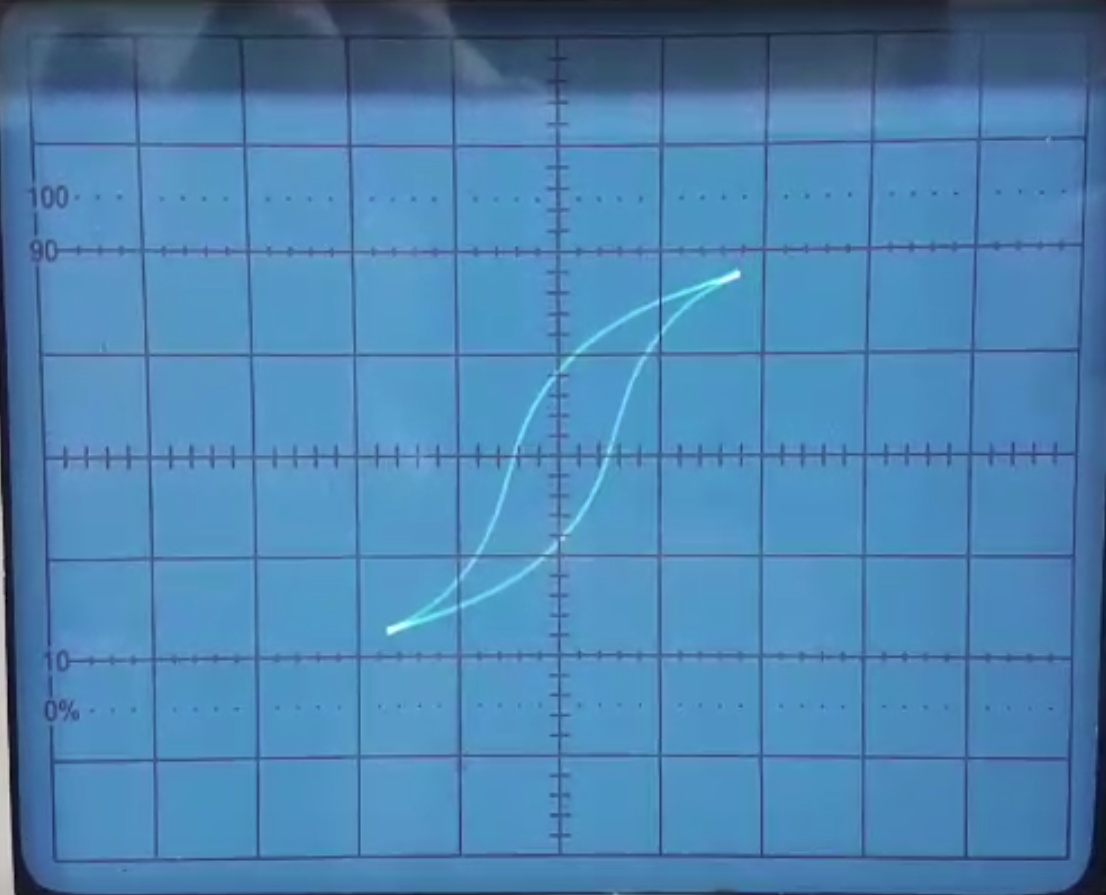
\includegraphics[width=0.8\linewidth]{PctFeSi}} \\Fe-Si
\end{minipage}
\hfill
\begin{minipage}[h]{0.31\linewidth}
\center{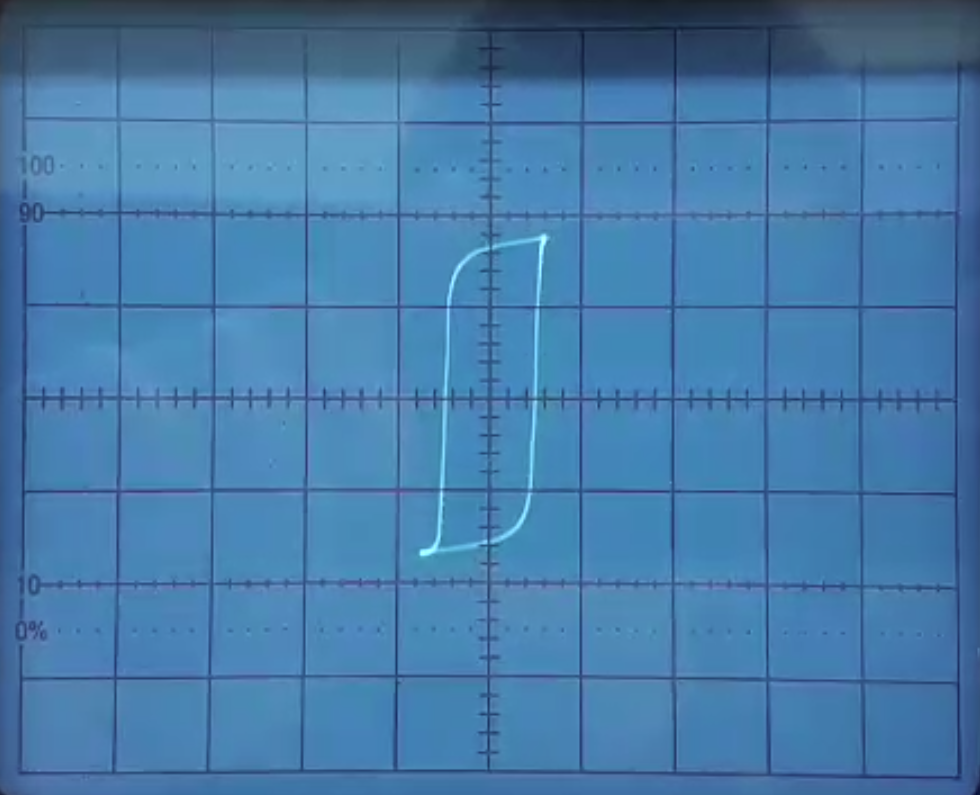
\includegraphics[width=0.8\linewidth]{PctPA}} \\Пермаллой
\end{minipage}
\hfill
\begin{minipage}[h]{0.31\linewidth}
\center{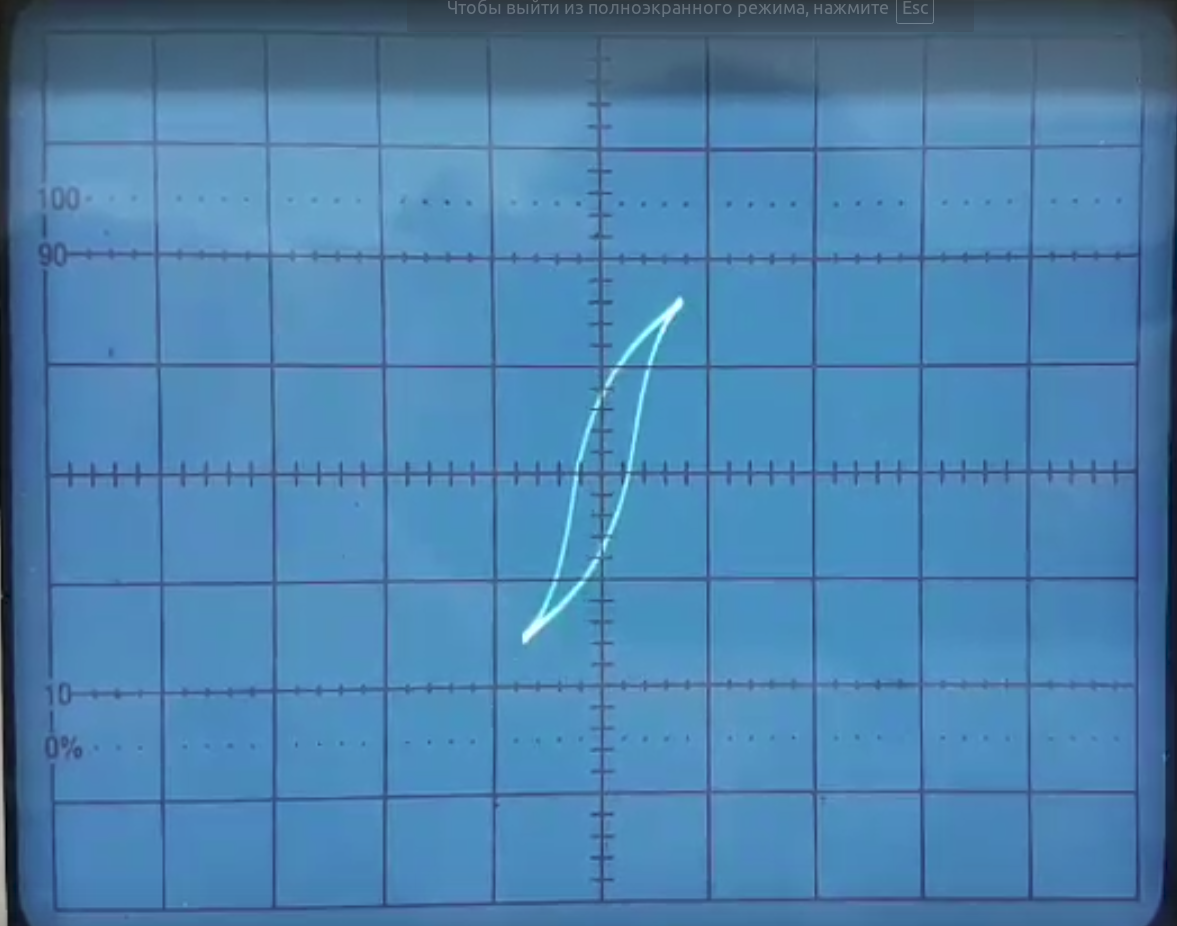
\includegraphics[width=0.8\linewidth]{PctFe}} \\Феррит
\end{minipage}
\vfill
\begin{minipage}[h]{0.31\linewidth}
\center{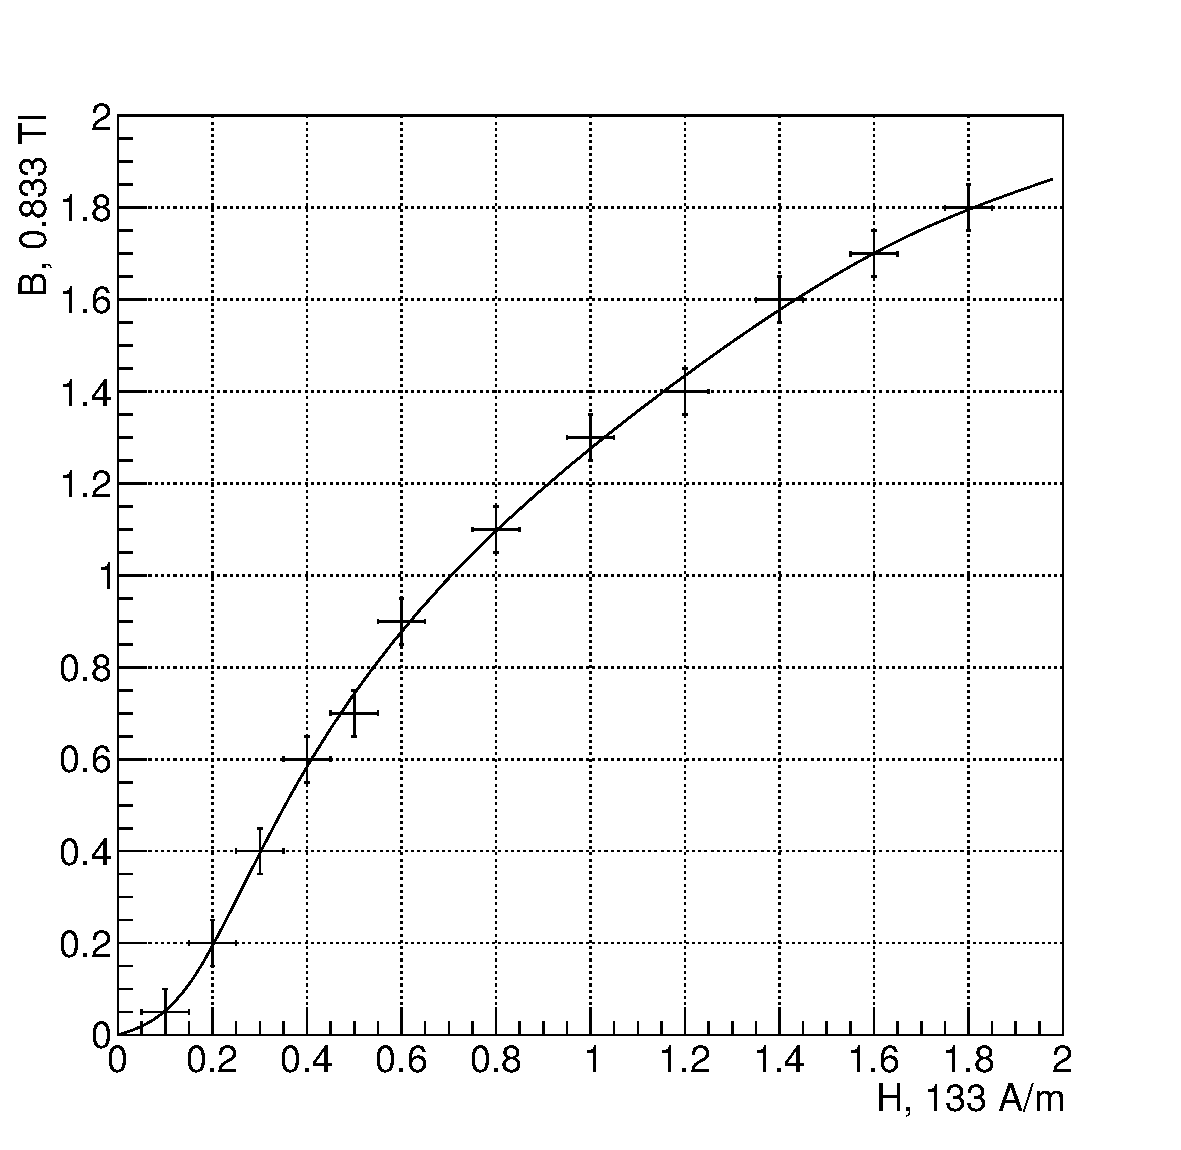
\includegraphics[width=0.8\linewidth]{FeSi}} \\Fe-Si 
\end{minipage}
\hfill
\begin{minipage}[h]{0.31\linewidth}
\center{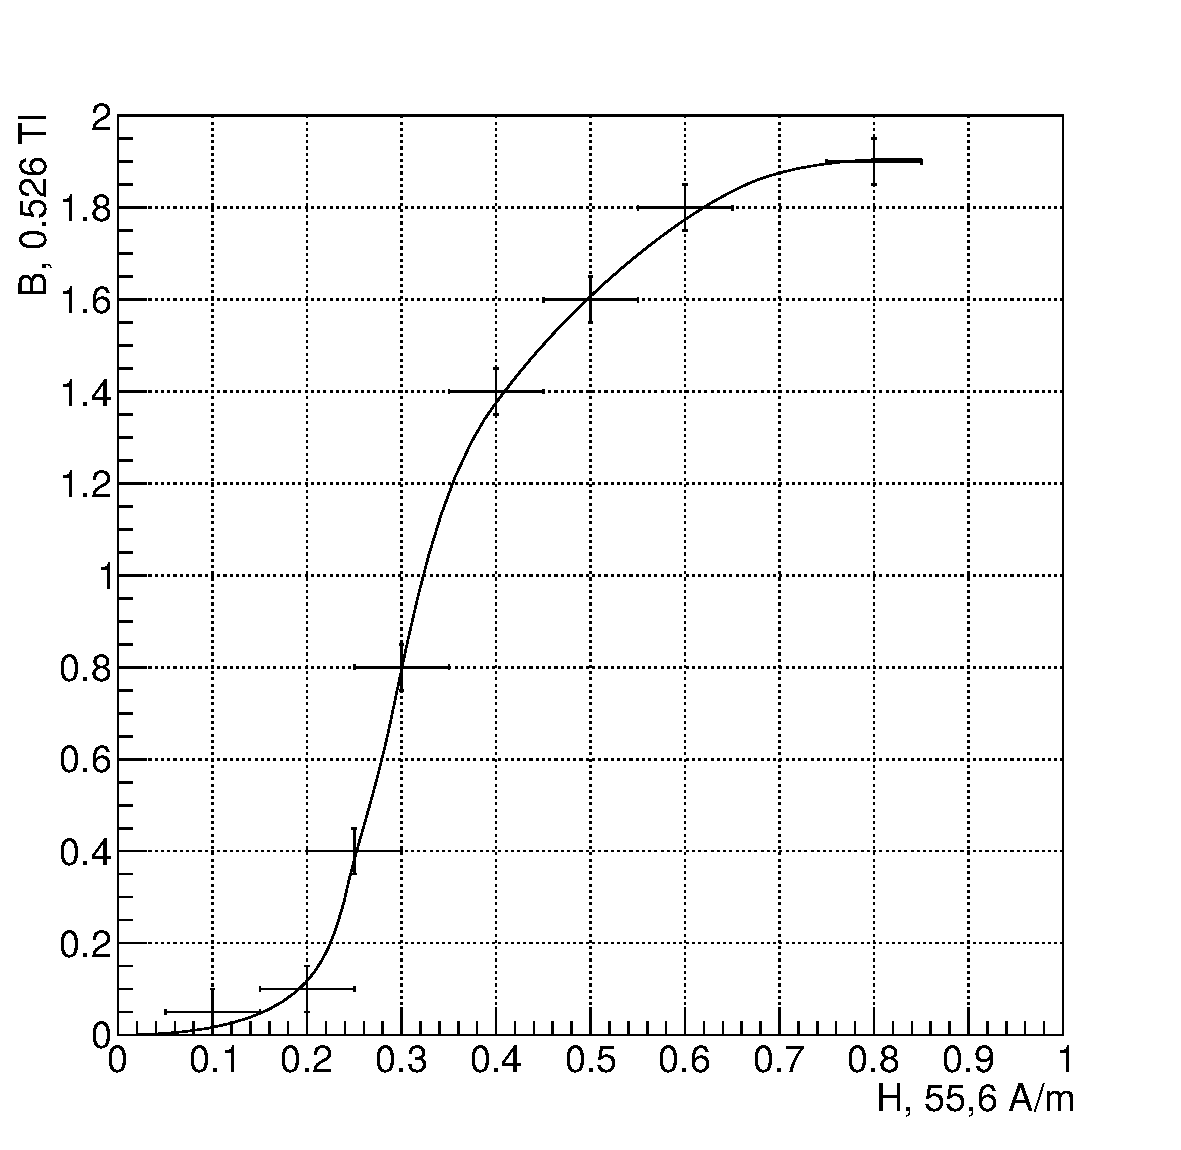
\includegraphics[width=0.8\linewidth]{PA}} \\Пермаллой
\end{minipage}
\hfill
\begin{minipage}[h]{0.31\linewidth}
\center{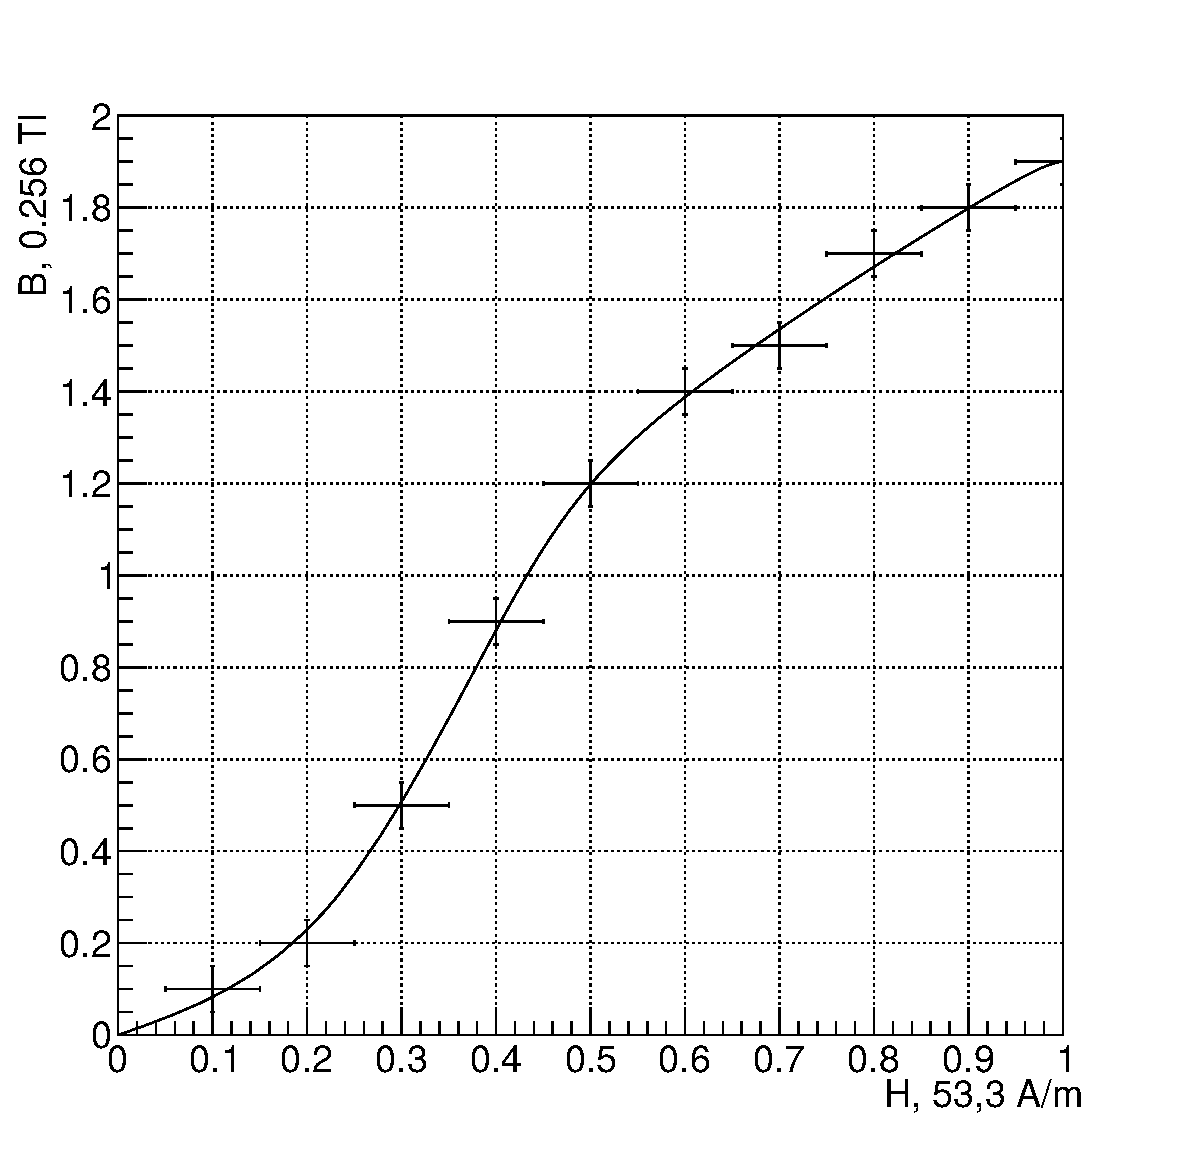
\includegraphics[width=0.8\linewidth]{Fer}} \\Феррит
\end{minipage}
\caption{Графическое представление экспериментальных данных}
\end{figure}
Отсюда легко получаем искомые величины (таблица 2):
\begin{table}[h]\centering
\begin{tabular}{c|c|c|c|}
~&Fe-Si&Пермаллой&Феррит\\
$H_c$, А/м&67$\pm$5&28$\pm$2&10$\pm$1\\
\hline
$B_r$, Тл&0,67$\pm$0,04&0,84$\pm$0,03&0,20$\pm$0,01\\
\hline
${\mu_\text{дифф}}_max$&20000&60000&15000\\
\hline
\end{tabular}
\caption{Характеристики образцов}
\end{table}
Здесь величины были вычислены по определениям с учетом известной цены деления, погрешность дифференциальной проницаемости не была посчитана, т.к. оценки довольно грубые (по 2 измеренным точкам, между которыми максимальный наклон).
\section{Вывод}
Цели работы были достигнуты, все величины были измерены. Хотя есть некоторые расхождения, значения, в целом, совпадают с табличными.
\end{document}